\documentclass{article}

\usepackage[letterpaper]{geometry}
\usepackage{amsmath}
\usepackage{amssymb}
\usepackage{siunitx}
\usepackage{graphicx}
\usepackage{tikz}
\usetikzlibrary{3d}

\title{4261 HW 5}
\author{Duncan Wilkie}
\date{?}

\newcommand{\Ba}[2]{\draw (#1,#2) circle (.25cm);\shade[ball color=red] (#1,#2) circle (.25cm);}
\newcommand{\Ti}[2]{\draw (#1,#2) circle (.25cm);\shade[ball color=green] (#1,#2) circle (.25cm);}
\newcommand{\Ox}[2]{\draw (#1,#2) circle (.25cm);\shade[ball color=blue] (#1,#2) circle (.25cm);}

\begin{document}

\maketitle

\section*{1a}
This is a face-centered cubic lattice.

\section*{1b}
Taking the origin to be the lower-left atom, we take the basis vectors $[\frac{1}{2},\frac{1}{2},0]a$, $[\frac{1}{2},0,\frac{1}{2}]a$, $[0,\frac{1}{2},\frac{1}{2}]a$, where $a$ is the lattice constant.
The atoms in the conventional cell that aren't at one of these basis vectors may be readily constructed from them.

\section*{1c}
Looking at the fcc conventional cell, it is evident that adjacent Zn atoms are spaced by the distance from the center of the face to the corner; in terms of the lattice constant, this is
\[
  \ell=a/\sqrt{2}=(\SI{0.54}{nm})/\sqrt{2}=\SI{0.38}{nm}
\]
The S atoms will be spaced by the same amount, since their primitive unit cell is that of the Zn atoms translated by $[1/4,1/4,-1/4]a$.
The Zn-S spacing is the magnitude of this translation,
\[\sqrt{3a^{2}/16}=a\sqrt{3}/4=(\SI{0.54}{nm})\sqrt{3}/4=\SI{0.23}{nm}\]

\section*{1d}
\begin{center}
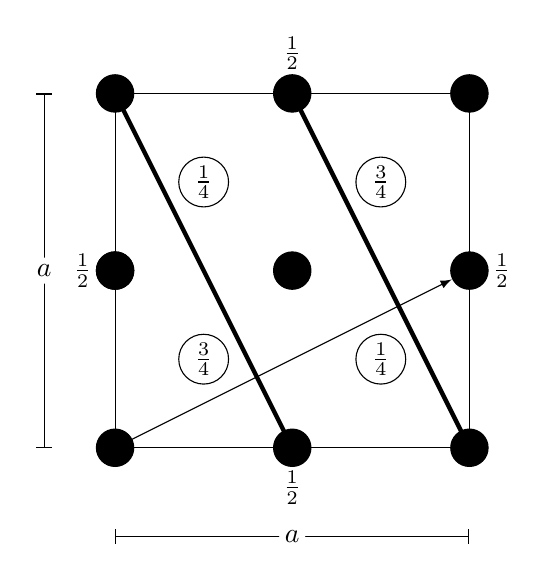
\begin{tikzpicture}[scale=4.5]
  \filldraw[black] (0,0) circle (1.5pt);
  \draw (0,0) -- (0.5,0);
  \filldraw[black] (0.5,0) circle (1.5pt) node[below,yshift=-5pt]{$\frac{1}{2}$};
  \draw (0.5,0) -- (1,0);
  \filldraw[black] (1,0) circle (1.5pt);
  \draw (1,0) -- (1,0.5);
  \filldraw[black] (1,0.5) circle (1.5pt) node[right,xshift=5pt]{$\frac{1}{2}$};
  \draw (1,0.5) -- (1,1);
  \filldraw[black] (1,1) circle (1.5pt);
  \draw (1,1) -- (0.5,1);
  \filldraw[black] (0.5,1) circle (1.5pt) node[above,yshift=5pt]{$\frac{1}{2}$};
  \draw (0.5,1) -- (0,1);
  \filldraw[black] (0,1) circle (1.5pt);
  \draw (0,1) -- (0,0.5);
  \filldraw[black] (0,0.5) circle (1.5pt) node[left,xshift=-5pt]{$\frac{1}{2}$};
  \draw (0,0.5) -- (0,0);
  \filldraw[black] (0,0.5) circle (1.5pt);

  \filldraw[black] (0.5,0.5) circle (1.5pt);

  \draw (0.25, 0.25) circle (2pt) node{$\frac{3}{4}$};
  \draw (0.25, 0.75) circle (2pt) node{$\frac{1}{4}$};
  \draw (0.75, 0.25) circle (2pt) node{$\frac{1}{4}$};
  \draw (0.75, 0.75) circle (2pt) node{$\frac{3}{4}$};


  \draw[|-|] (0,-0.25) -- (1,-0.25);
  \filldraw[white] (0.5,-0.25) circle (1pt);
  \node at (0.5,-0.25) (a) {$a$};

  \draw[|-|] (-0.2,0) -- (-0.2,1);
  \filldraw[white] (-0.2,0.5) circle (1pt);
  \node at (-0.2,0.5) (a) {$a$};

  \draw[-latex] (0,0) -- (0.95,0.475);


  \draw[ultra thick] (0,1) -- (0.5,0);
  \draw[ultra thick] (0.5,1) -- (1,0);

\end{tikzpicture}
\end{center}
Note that the arrow lies parallel to the $xy$-plane and the lattice planes are pointing out of the page from the lines representing them.

\section*{1e}
Notice from the image that the arrow representing the given direction has length $\sqrt{a^{2}+a^{2}/4}=a\sqrt{5}/2$, and along its length
there are two and a half instances of the lattice plane spacing. The spacing between planes is then $a\sqrt{5}/25$.

\section*{2}
A crystal plane is a plane overlaying a crystalline lattice that intersects at least three non-collinear points of the lattice.
Miller indices describe lattice planes by first constructing a reciprocal-space basis corresponding to a direct-space basis
of choice, and denoting points of the reciprocal lattice by $(hkl)$ where the numbers are the coefficients of the linear combination of
the reciprocal basis vectors that equals the point.
This represents a lattice plane by the one-to-one correspondence between reciprocal vectors and lattice planes normal to them.

The reciprocal lattice vector has components $b_{i}=2\pi/a_{i}$, and the family of lattice planes $(hkl)$ is normal to the reciprocal
lattice vector with components $h$, $k$, and $l$, so it will also be normal to the direct lattice vector $[hkl]$ since the relation
between the components is simply a constant multiplication.
For an orthorhombic crystal, the expression of the reciprocal lattice vector components above doesn't hold, so the overall result fails.
We have
\[
  d_{(hkl)}=\frac{2\pi}{|\vec{G}|}=\frac{2\pi}{\sqrt{h^{2}|b_{1}|^{2}+k_{2}|b_{2}|^{2}+l^{2}|b_{3}|^{2}}}
  \Leftrightarrow \frac{1}{d_{(hkl)}^{2}}=\frac{h^{2}|b_{1}|^{2}+k^{2}|b_{2}|^{2}+l^{2}|b_{3}|^{2}}{(2\pi)^{2}}
\]
Since for orthogonal axes $|b_{i}|=2\pi/|a_{i}|\Leftrightarrow |b_{i}|^{2}/(2\pi)^{2}=1/|a_{i}|^{2}$, this becomes
\[
  \frac{1}{d^{2}_{(hkl)}}=h^{2}/|a_{1}|^{2}+k^{2}/|a_{2}|^{2}+l^{2}/|a_{3}|^{2}
  \Leftrightarrow d_{(hkl)}=\frac{1}{\sqrt{h^{2}/|a_{1}|^{2}+k^{2}/|a_{2}|^{2}+l^{2}/|a_{3}|^{2}}}
\]
which for $|a_{1}|=|a_{2}|=|a_{3}|=a$ becomes the desired
\[
  d_{(hkl)}=\frac{a}{\sqrt{h^{2}+k^{2}+l^{2}}}
\]

\section*{3a}
The reciprocal lattice conjugate to a given direct lattice $\vec{R}$ is the collection of points $\vec{G}$ such that
\[
  e^{i\vec{G}\cdot\vec{R}}=1
\]

\section*{3b}
We write ${a}_{1}=x_{1}\hat{x}=y_{1}\hat{y}+z_{1}\hat{z}$ and so on. We then compute
\[
  {a_{2}\times a_{3}}=
  \begin{vmatrix}
    \hat{x} & \hat{y} & \hat{z} \\
    x_{2} & y_{2} & z_{2} \\
    x_{3} & y_{3} & z_{3}
  \end{vmatrix}
  =(y_{2}z_{3}-z_{2}y_{3})\hat{x}+(z_{2}x_{3}-x_{2}z_{3})\hat{y}+(x_{2}y_{3}-y_{2}x_{3})\hat{z}
\]
\[
  a_{1}\cdot(a_{2}\times a_{3})
  =x_{1}(y_{2}z_{3}-z_{2}y_{3})+y_{1}(z_{2}x_{3}-x_{2}z_{3})+z_{1}(x_{2}y_{3}-y_{2}x_{3})
\]
\[
  b_{1}=2\pi\frac{(y_{2}z_{3}-z_{2}y_{3})\hat{x}+(z_{2}x_{3}-x_{2}z_{3})\hat{y}+(x_{2}y_{3}-y_{2}x_{3})\hat{z}}
  {x_{1}(y_{2}z_{3}-z_{2}y_{3})+y_{1}(z_{2}x_{3}-x_{2}z_{3})+z_{1}(x_{2}y_{3}-y_{2}x_{3})}
\]
Dotting this by $a_{1}$ will yield $a_{1}\cdot b_{1}=1\Rightarrow e^{i\vec{G}\cdot\vec{R}}=e^{i2\pi}=1$.
For the other cases,
\[
  {a_{3}\times a_{1}}=
  \begin{vmatrix}
    \hat{x} & \hat{y} & \hat{z} \\
    x_{3} & y_{3} & z_{3} \\
    x_{1} & y_{1} & z_{1}
  \end{vmatrix}
  =(y_{3}z_{1}-z_{3}y_{1})\hat{x}+(z_{3}x_{1}-x_{3}z_{1})\hat{y}+(x_{3}y_{1}-y_{3}x_{1})\hat{z}
\]
\[
  {a_{1}\times a_{2}}=
  \begin{vmatrix}
    \hat{x} & \hat{y} & \hat{z} \\
    x_{1} & y_{1} & z_{1} \\
    x_{2} & y_{2} & z_{2}
  \end{vmatrix}
  =(y_{1}z_{2}-z_{1}y_{2})\hat{x}+(z_{1}x_{2}-x_{1}z_{2})\hat{y}+(x_{1}y_{2}-y_{1}x_{2})\hat{z}
\]
In each case, it is evident dotting by $a_{2}$ and $a_{3}$ respectively will yield 1, proving that the given vectors are reciprocal
to the direct principal lattice vectors.
For 2d, we can take $a_{3}=\hat{z}$, yielding
\[
  b_{1}=2\pi\frac{a_{2}\times\hat{z}}{a_{1}\cdot(a_{2}\times \hat{z})}
\]
\[
  b_{2}=2\pi\frac{\hat{z}\times a_{1}}{a_{1}\cdot(a_{2}\times \hat{z})}
\]
The expression for $b_{3}$ is discarded because it is not in the $x-y$ plane.

\section*{3c}
Tetragonal lattices are those with conventional unit cells containing all right angles with only two side lengths equal.
Orthorhombic lattices are those with conventional unit cells containing all right angles with no two side lengths equal.
Writing the orthorhombic lattice vectors as $\vec{a}_{1}=a_{1}\hat{x}$, $\vec{a}_{2}=a_{2}\hat{y}$, and $\vec{a}_{3}=a_{3}\hat{z}$,
we compute via the formula for the reciprocal lattice vectors
\[
  b_{1}=2\pi\frac{a_{2}a_{3}\hat{x}}{a_{1}a_{2}a_{3}}=\frac{2\pi}{a_{1}}\hat{x}
\]
\[
  b_{2}=2\pi\frac{a_{3}a_{1}\hat{y}}{a_{1}a_{2}a_{3}}=\frac{2\pi}{a_{2}}\hat{y}
\]
\[
  b_{3}=2\pi\frac{a_{1}a_{2}\hat{z}}{a_{1}a_{2}a_{3}}=\frac{2\pi}{a_{3}}\hat{z}
\]
Taking the magnitude of a reciprocal vector
\[
  \vec{G}=hb_{1}+kb_{2}+lb_{3}=h\frac{2\pi}{a_{1}}\hat{x}+k\frac{2\pi}{a_{2}}\hat{y}+l\frac{2\pi}{a_{3}}\hat{z}
\]
we have
\[
  |\vec{G}|=2\pi\sqrt{h^{2}/a_{1}^{2}+k^{2}/a_{2}^{2}+l^{2}/a_{3}^{2}}
\]
The result of the last part of problem 2 identifies the square root term as $\frac{1}{d}$, from which the result is immediate.

\section*{4a}
The reciprocal lattice vectors are, since the direct lattice vectors are orthogonal,
\[
  b_{1}=\frac{2\pi}{\SI{0.468}{nm}}=\SI{13.4}{nm^{-1}}
\]
and
\[
  b_{2}=\frac{2\pi}{\SI{0.342}{nm}}=\SI{18.4}{nm^{-1}}
\]

Correspondingly, we can sketch the lattice with Miller indices $(h,k)$ indicated as
\begin{center}
  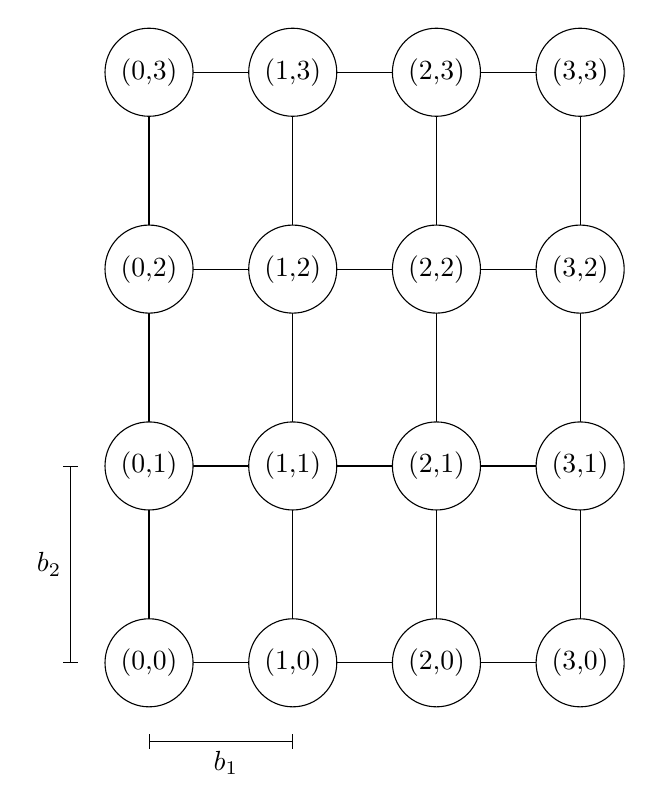
\begin{tikzpicture}[scale=2.5]
    \draw[xscale=0.73] (0,0) grid (3,3);
    \draw[|-|] (0,-.4) -- (0.73,-.4) node[yshift=-0.27cm, xshift=-.85cm] {$b_{1}$};
    \draw[|-|] (-.4,0) -- (-.4,1) node[yshift=-1.25cm, xshift=-0.27cm] {$b_{2}$};

    \foreach \h in {0, 1, 2, 3}
    \foreach \k in {0, 1, 2, 3}
    \node[circle,draw,fill=white] at (\h*0.73, \k){(\h,\k)};
  \end{tikzpicture}
\end{center}

\section*{4b}
The Laue condition states that $\vec{k}-\vec{k'}=\vec{G}$, and conservation of energy restricts $|\vec{k}|=|\vec{k'}|$.
The wave number of the incident light is therefore $|\vec{k}|=|\vec{k'}|=\frac{2\pi}{\SI{0.166}{nm}}=\SI{37.9}{nm^{-1}}$.
For $(210)$ diffraction, the Laue condition implies $\Delta k=\vec{k}-\vec{k'}=(210)$, which, eliding the Miller indices for clarity,
can be drawn as
\begin{center}
  \begin{tikzpicture}[scale=2.5]
    \draw[xscale=0.73] (0,0) grid (3,3);
    \draw[|-|] (0,-.4) -- (0.73,-.4) node[yshift=-0.27cm, xshift=-.85cm] {$b_{1}$};
    \draw[|-|] (-.4,0) -- (-.4,1) node[yshift=-1.25cm, xshift=-0.27cm] {$b_{2}$};


    \draw[-latex] (0,0) -- (1.46,1) node[xshift=-.3cm, yshift=-.4cm] {$\vec{G}$};
    \draw[-latex] (0,0) -- (-0.2,1.8) node[xshift=-.3cm, yshift=-.4cm] {$\vec{k'}$};
    \draw[-latex] (1.46,1) -- (-0.2,1.8) node[xshift=.3cm, yshift=.2cm] {$\vec{k}$};
  \end{tikzpicture}
\end{center}

\section*{4c}
Consider a unit cell containing two atoms.
The Wigner-Seitz construction involves drawing the perpendicular bisectors of the vector between the point at the center and
the points at the edge (dark lines denoting bisectors):
\begin{center}
  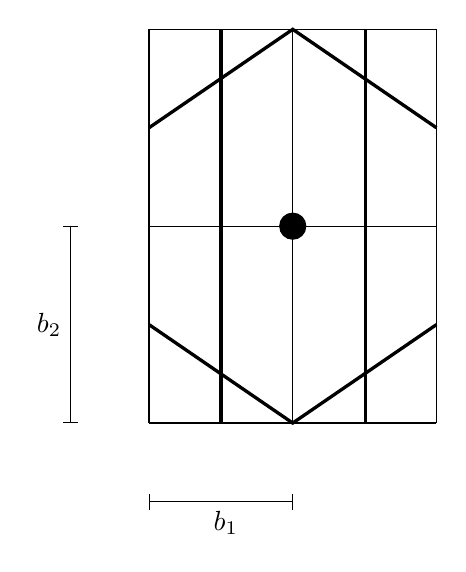
\begin{tikzpicture}[scale=2.5]
    \draw[xscale=0.73] (0,0) grid (2,2);
    \node[circle,draw,fill] at (0.73,1) {};
    \draw[|-|] (0,-.4) -- (0.73,-.4) node[yshift=-0.27cm, xshift=-.85cm] {$b_{1}$};
    \draw[|-|] (-.4,0) -- (-.4,1) node[yshift=-1.25cm, xshift=-0.27cm] {$b_{2}$};
    \draw[very thick] (0,1.5) -- (0.73,2) -- (1.46,1.5);
    \draw[very thick] (0,.5) -- (0.73,0) -- (1.46,.5);

    \draw[very thick] (0.365,0) -- (0.365,2);
    \draw[very thick] (1.1,0) -- (1.1,2);
  \end{tikzpicture}
\end{center}
The regions where it takes a minimum of zero proper edge crossings to reach the point at the center is the first Brillouin zone;
that where it takes one crossing, the second, etc.:
\begin{center}
  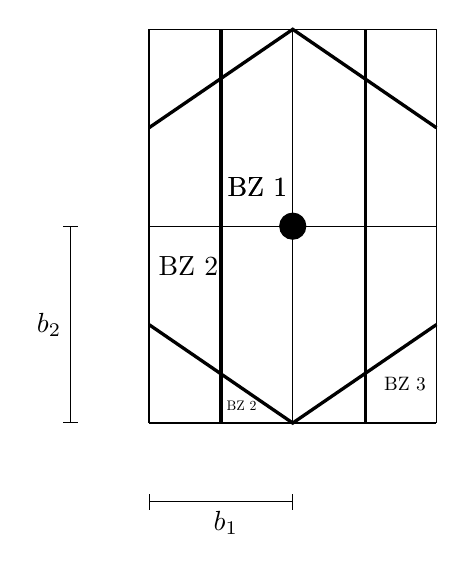
\begin{tikzpicture}[scale=2.5]
    \draw[xscale=0.73] (0,0) grid (2,2);
    \node[circle,draw,fill] at (0.73,1) {};
    \draw[|-|] (0,-.4) -- (0.73,-.4) node[yshift=-0.27cm, xshift=-.85cm] {$b_{1}$};
    \draw[|-|] (-.4,0) -- (-.4,1) node[yshift=-1.25cm, xshift=-0.27cm] {$b_{2}$};
    \draw[very thick] (0,1.5) -- (0.73,2) -- (1.46,1.5);
    \draw[very thick] (0,.5) -- (0.73,0) -- (1.46,.5);

    \draw[very thick] (0.365,0) -- (0.365,2);
    \draw[very thick] (1.1,0) -- (1.1,2);

    \node at (0.55, 1.2) {BZ 1};
    \node at (0.2, .8) {BZ 2};
    \node at (0.55, 1.2) {BZ 1};
    \node[scale=.5] at (0.47, .09) {BZ 2};
    \node[scale=.7] at (1.3,.2) {BZ 3};
  \end{tikzpicture}
\end{center}

\section*{5}
Some clever Tikz hacking yields
\begin{center}
  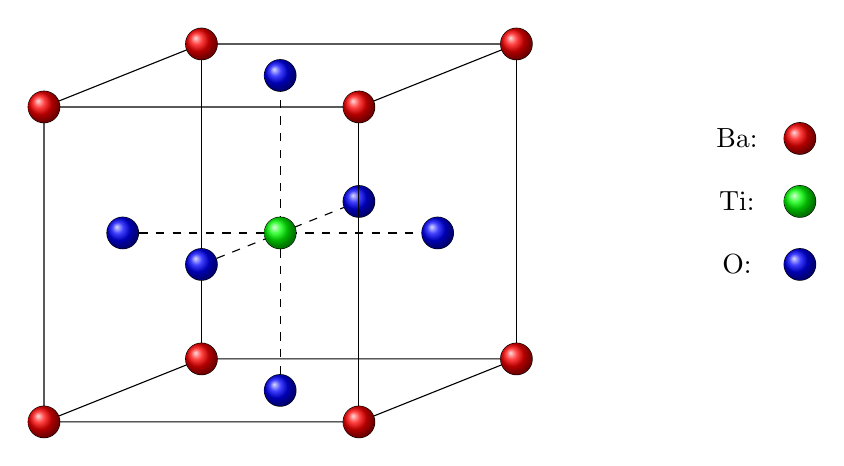
\begin{tikzpicture}[scale=.8]
    \draw (0,0) -- (5,0) -- (7.5,1) -- (2.5,1) -- (0,0) -- (0,5) -- (2.5,6) -- (7.5,6) -- (5,5) -- (0,5);
    \draw (2.5,1) -- (2.5,6);
    \draw[dashed] (2.5,2.5) -- (5,3.5);
    \draw[dashed] (1.25,3) -- (6.25,3);
    \draw[dashed] (3.75,.5) -- (3.75,5.5);
    \Ox{5}{3.5}
    \draw (5,5) -- (5,0);
    \draw (7.5,1) -- (7.5,6);

    \Ba{0}{0}
    \Ba{5}{0}
    \Ba{0}{5}
    \Ba{5}{5}
    \Ba{2.5}{1}
    \Ba{7.5}{1}
    \Ba{2.5}{6}
    \Ba{7.5}{6}

    \Ox{5/2}{5/2}
    \Ox{1.25}{3}
    \Ox{6.25}{3}
    \Ox{3.75}{5.5}
    \Ox{3.75}{.5}

    \Ti{3.75}{3}

    \node[xshift=-.8cm] at (12,4.5) {Ba:};
    \Ba{12}{4.5}
    \node[xshift=-.8cm] at (12, 3.5) {Ti:};
    \Ti{12}{3.5}
    \node[xshift=-.8cm] at (12, 2.5) {O:};
    \Ox{12}{2.5}

  \end{tikzpicture}
\end{center}
Applying the definition of the structure factor,
\[
  S_{(00l)}f_{Ba}(00l)\sum_{\textrm{Ba atoms at }\vec{x}_{j}}e^{i(00l)\cdot \vec{x}_{j}}
  +f_{Ti}(00l)\sum_{\textrm{Ti atoms at }\vec{x}_{j}}e^{i(00l)\cdot \vec{x}_{j}}
  +f_{O}(00l)\sum_{\textrm{O atoms at }\vec{x}_{j}}e^{i(00l)\cdot \vec{x}_{j}}
\]
\[
  =  f_{Ba}(00l)\sum_{\textrm{Ba atoms at }z_{j}}e^{2\pi ilz_{j}}
  +f_{Ti}(00l)\sum_{\textrm{Ti atoms at }z_{j}}e^{2\pi ilz_{j}}
  +f_{O}(00l)\sum_{\textrm{O atoms at }z_{j}}e^{2\pi ilz_{j}}
\]
Since $(00l)$ is a reciprocal lattice vector, and $x_{j}$ is a direct lattice vector for the barium atom, the first sum equals one.
For the titanium atom, since $z_{j}$ is half that of the direct lattice vector $z_{j}'=1$, so
$e^{2\pi ilz_{j}}=e^{2\pi ilz'_{j}/2}=(e^{\pi iz'_{j}})^{l}=(-1)^{l}$, proving the form of the second term.
For the oxygen atoms, one of them has $z_{j}=0$, so the exponential term is one; the other two have the same $z_{j}$ as titanium, leaving
the final result
\[
  S_{(00l)}=f_{Ba}+(-1)^{l}f_{Ti}+(1+2(-1)^{l})f_{O}
\]
Using $I_{(hkl)}\propto M_{(hkl)}|S_{(hkl)}|^{2}$, and the fact that the multiplicities for all $(00l)$ are identical
(there are six identically-spaced families of planes in every case), we can write
\[
  \frac{I_{(002)}}{I_{(001)}}=\frac{[f_{Ba}+f_{Ti}+3f_{O}]^{2}}{[f_{Ba}-f_{Ti}-f_{O}]^{2}}
  \approx \frac{c^{2}[Z_{Ba}+Z_{Ti}+3Z_{O}]^{2}}{c^{2}[Z_{Ba}-Z_{Ti}-Z_{O}]^{2}}
  =\frac{[56+22+3\cdot8]^{2}}{[56-22-8]^{2}}
  =15.4
\]


\end{document}
%%% Local Variables:
%%% mode: latex
%%% TeX-master: t
%%% End:
